\documentclass[10pt,twocolumn]{article}

% ---------------------------------------------------------------------------
% ironrun: Sealed Execution for LLM Coding Agents
% Build:  make -C paper        Reproduce numbers:  go run ./paper/eval
% ---------------------------------------------------------------------------

\usepackage[T1]{fontenc}
\usepackage[utf8]{inputenc}
\usepackage{amsmath,amsthm}
\usepackage{libertine}
\usepackage[libertine]{newtxmath}
\usepackage[scaled=0.92]{inconsolata}
\usepackage[letterpaper,margin=0.75in,columnsep=0.28in]{geometry}
\usepackage{microtype}
\usepackage{xcolor}
\usepackage{booktabs}
\usepackage{multirow}
\usepackage{tabularx}
\usepackage{threeparttable}
\usepackage{enumitem}
\usepackage{algorithm}
\usepackage[noend]{algpseudocode}
\usepackage{tikz}
\usetikzlibrary{arrows.meta,positioning,fit,backgrounds,calc,shapes.geometric,decorations.pathreplacing}
\usepackage{pgfplots}
\pgfplotsset{compat=1.17}
\usepackage{caption}
\usepackage[numbers,sort&compress]{natbib}
\usepackage[hidelinks,breaklinks]{hyperref}
\usepackage[capitalise,nameinlink]{cleveref}

\definecolor{ink}{HTML}{1F2933}
\definecolor{accent}{HTML}{0B6E4F}
\definecolor{warn}{HTML}{B54708}
\definecolor{soft}{HTML}{EEF2F6}
\definecolor{secret}{HTML}{C2410C}

\newcommand{\sys}{\textsf{ironrun}}
\newcommand{\code}[1]{\texttt{\upshape\detokenize{#1}}}
\newcommand{\red}{\texttt{[REDACTED]}}
\newtheorem{property}{Property}
\newtheorem{observation}{Observation}

\setlist{nosep,leftmargin=1.2em}
\captionsetup{font=small,labelfont=bf}
\setlength{\abovecaptionskip}{4pt}

\hypersetup{
  pdftitle={Sealed Execution: Letting LLM Coding Agents Use Credentials Without Seeing Them},
  pdfauthor={Mihir Gupta, Stephen Keehn},
}

\title{\Large\bfseries Sealed Execution: Letting LLM Coding Agents\\Use Credentials Without Seeing Them}
\author{%
  Mihir Gupta \qquad Stephen Keehn\\[2pt]
  \normalsize Generalized Labs\\
  \normalsize\url{https://github.com/Generalized-Labs/ironrun}}
\date{}

\begin{document}
\maketitle

% ===========================================================================
\begin{abstract}
LLM coding agents run shell commands, and whatever those commands print
becomes model context. A credential that surfaces in output---through
\code{printenv}, a verbose \code{curl}, or a stack trace that embeds a
connection string---is sent to the model provider, persisted in local session
transcripts, and must be rotated. We present \sys{}, an open-source runtime that
turns the agent's tool boundary into a one-way valve: secret values flow
\emph{into} child processes as environment variables or temporary files, but
not back \emph{out}. \sys{} combines (i)~value-blind agent interfaces exposed over
the Model Context Protocol, (ii)~human authorization tiers bound to a single
agent session, environment, and expiry, (iii)~a streaming known-value redactor
with whitespace-tolerant, fragment, and alignment-aware encoding matching under
a bounded hold-back, and (iv)~defense-in-depth containment: network
namespaces or Seatbelt, a seccomp denylist, core-dump suppression,
process-group lifetime control, CI fork gating, and a hash-chained audit log.
We report an adversarial self-audit of the 16.6\,kLOC Go implementation that
confirmed 49 distinct defects---2 critical and 6 high severity, 44 now fixed---among them a YAML-injection path that let an agent
smuggle commands past human review and a CLI command that printed the vault
root key, together with their fixes. On a corpus of 21 output transformations
$\times$ 6 credential formats driven through the real execution path, the
number of cases that leak at least half of a secret falls from 52 to 28; for
transformations produced by ordinary tools it falls from 21 of 72 to 3 of 72, all
three involving a 12-byte password below the fragment threshold. The residue
consists of deliberate transformations that no known-value redactor can catch. \sys{} adds about 0.1\,ms to spawning a command
(7\,ms with macOS network isolation), and its redactor sustains 13--35\,MB/s. We argue that redaction is the right safety net for
\emph{accidental} disclosure, while authorization and isolation must bound
\emph{deliberate} exfiltration, and we make the limits of each explicit.
\end{abstract}

% ===========================================================================
\section{Introduction}
\label{sec:intro}

Coding agents such as Claude Code, Codex, and Cursor operate by issuing tool
calls---most importantly, shell commands---and reading their output. That
output is appended to the model's context window, transmitted to the model
provider on every subsequent turn, and typically persisted by the agent host as
a local transcript (Claude Code, for example, stores JSONL session logs under
\code{~/.claude/projects/}). Anything a command prints is therefore
\emph{published}: to the provider, to the transcript store, and to anyone who
later reads, shares, or screen-records the session.

Credentials reach output through utterly ordinary debugging. An agent asked to
fix a failing integration test may run \code{printenv} to check configuration,
\code{cat .env} to inspect it, \code{curl -v} to reproduce an HTTP error (which
echoes the \code{Authorization} header), or simply rerun a test whose failure
message embeds the database URL. Each of these discloses a secret the human
never intended to share, and because transcripts cannot be retracted from a
provider's logs, the only safe response is rotation. Practitioners report this
happening repeatedly in normal use~\citep{cc_issue64326,cc_issue32523},
and a recent study of 17{,}022 agent skills attributes 73.5\% of credential leaks
to debug output that agent frameworks feed back into model
context~\citep{chen2026skillsleak}. Once a value has entered context it also
resurfaces in places transcript scrubbing cannot reach, such as reasoning
traces~\citep{panfilov2026reasoning}.

Existing tools each cover part of the problem. Secret managers' \code{run}
wrappers inject values into a child's environment~\citep{onepassword_oprun,doppler_cli,infisical_run};
1Password's also conceals values in the child's output, but none of them
mediates \emph{which} commands an agent may run with which secrets. Agent-host
deny rules that hide \code{.env} files do not stop commands that read the file
indirectly~\citep{claudecode_permissions,munis2025knostic,eve2026env}. Credential
brokers control \emph{who may authenticate}~\citep{onepassword2026unified,bitwarden2026agentaccess},
not \emph{what a command prints after authenticating}. Proxy-substitution
designs never give the process the real value at all, but apply only to HTTP(S)
traffic through a TLS-terminating proxy~\citep{claudecode_sandboxing,infisical_agentproxy,flyio_tokenizer}.
CI runners have long masked known secrets and their encodings in job
logs~\citep{githubrunner2019encoders,github2026secureuse}, and agent-side tools
have recently begun to scrub tool output by literal
matching~\citep{fnox_mcp,prismor2026}. What is missing is a design---and an
evaluation---that combines these at the agent's tool boundary for arbitrary
command-line programs: database clients, test runners, \code{kubectl},
\code{terraform}.

\paragraph{Insight.} The agent needs the \emph{effect} of a credential---a
passing test, a successful deploy---not its \emph{value}. If the same component
that resolves and injects secrets also mediates the command's output, then
redaction becomes a problem over \emph{known} values rather than a detection
problem over unknown ones. Known-value redaction is deterministic, has no
false negatives for literal occurrences, and can be extended systematically to
the encodings that ordinary tools apply.

\paragraph{Contributions.}
\begin{itemize}
\item A threat model for credential disclosure through agent tool output that
  separates \emph{accidental} disclosure, \emph{prompt-injected} agents acting
  through their tools, and hostile same-user code (\cref{sec:threat}).
\item The design and implementation of \sys{}, an MIT-licensed local runtime
  comprising value-blind MCP interfaces, session-bound tiered authorization with
  in-place continuation, a streaming redactor with a proved chunking-invariance
  property, and layered containment (\cref{sec:design,sec:impl}).
\item An adversarial self-audit of the implementation, its findings, and the
  lessons they teach about where such systems fail: in the text-rendering and
  state surfaces around the cryptography, not in the cryptography
  (\cref{sec:audit}).
\item To our knowledge the first adversarial evaluation of known-value redaction
  at an agent's tool boundary: a 126-case leak corpus driven through the real
  execution path and attacked with a decoder battery, plus false-positive and
  overhead measurements, with an open harness (\cref{sec:eval}).
\end{itemize}

% ===========================================================================
\section{Background}
\label{sec:background}

\paragraph{Agent tool loops.} An agent host repeatedly sends the conversation
to a model, receives tool calls, executes them locally, and appends results.
The Model Context Protocol (MCP)~\citep{mcp2026spec} standardizes how a host
discovers and invokes local tool servers over stdio. Every byte a tool returns
becomes model input, is retained for the rest of the session, and is commonly
written to disk by the host.

\paragraph{Why output is the hard channel.} Secrets can leave through three
channels: \emph{inputs} the agent writes (a value typed into a command line),
\emph{outputs} a command prints, and \emph{side effects} (network, files). The
first is solvable by never giving the agent the value; the third is the
domain of sandboxes. The second is the subtle one: an agent that has never
seen a credential can still cause it to be printed, merely by running the
program that uses it. Rotation is the only remedy after the fact.

\paragraph{Scenarios.} Three representative accidents motivate the design:
(1)~a connection failure prints a DSN with an embedded password;
(2)~\code{curl -v -u deploy:$TOKEN} prints
\code{Authorization: Basic} followed by the base64 of \code{deploy:<token>};
(3)~\code{docker compose config} prints the interpolated environment. In (2)
the token never appears literally---it appears base64-encoded \emph{at a byte
offset that depends on the username}, a case that matters in \cref{sec:eval}.

% ===========================================================================
\section{Threat Model}
\label{sec:threat}

\paragraph{Principals.} The \emph{operator} is the human developer; they are
trusted, author the policy, and approve access. The \emph{agent} is the model
together with its host; it is trusted to act on the operator's behalf but may
be mistaken or manipulated. \emph{Child commands} are the operator's own build,
test, and deploy programs, run on the agent's request. The \emph{model provider}
receives everything in context and is outside the operator's control.

\paragraph{Adversaries.} We distinguish three:
\begin{itemize}
\item[\textbf{A1}] \textbf{Accidental disclosure.} An honest agent runs
  ordinary commands that happen to print secrets. This is the common case and
  the primary target.
\item[\textbf{A2}] \textbf{Manipulated agent.} A prompt-injected or misaligned
  agent~\citep{greshake2023youve} tries to move a secret into its context or
  off the machine, but acts only through its tools: MCP calls, its native shell,
  and file edits.
\item[\textbf{A3}] \textbf{Hostile same-user code.} Arbitrary native code
  running as the operator's UID. It can read the user's keychain, attach to
  processes where the OS permits, and rewrite user-owned files. A3 is out of
  scope; containing it requires a separate OS user, container, or VM.
\end{itemize}

\paragraph{Goals.}
\begin{itemize}
\item[\textbf{G1}] \textbf{Value-blindness.} No \sys{} interface reachable by the
  agent---MCP tools, CLI, local API, daemon, audit log---returns a secret value or
  key material.
\item[\textbf{G2}] \textbf{Output confidentiality.} When an authorized child
  prints a secret it was given, in literal form or a common encoding, the agent
  receives a placeholder instead.
\item[\textbf{G3}] \textbf{Least authority.} The agent obtains secret-bearing
  execution only for commands and environments a human approved, bound to one
  agent session and an expiry; revocation takes effect on the next call.
\item[\textbf{G4}] \textbf{Containment.} By default a secret-bearing command
  has no network, cannot trace other processes, cannot dump core, and cannot
  outlive its time budget.
\item[\textbf{G5}] \textbf{Accountability.} Every run leaves a tamper-evident
  record of what ran with which secret \emph{names}.
\end{itemize}

\paragraph{Non-goals.} \sys{} does not attempt to stop an authorized process
that \emph{deliberately} transforms a secret with an arbitrary function before
printing it (\cref{obs:arbitrary}); does not defend against A3; does not remove
data from provider logs; and does not guarantee physical erasure of temporary
file secrets on SSDs or copy-on-write filesystems.

\paragraph{A note on A2 and the native shell.} Agent hosts typically give the
agent its own unrestricted shell in addition to any MCP server. \sys{} removes
secrets from the agent's ambient environment and from the repository, which
defeats A1 and casual A2 (\code{printenv}, \code{cat .env}). But a determined A2
with an unrestricted same-user shell approaches A3: on macOS, for instance, a
keychain item created through \code{/usr/bin/security} is readable by any
process that invokes the same binary. Deployments that face A2 must therefore
pair \sys{} with the host's own command restrictions or sandbox, or run \sys{}'s
state under a separate user. We return to this in \cref{sec:discussion}.

% ===========================================================================
\section{Design}
\label{sec:design}

\Cref{fig:arch} shows the architecture. All entry points---CLI, MCP server, TUI,
and a local Unix-socket API---converge on a single execution core, so that
authorization, resolution, containment, redaction, and audit cannot diverge
between surfaces.

\begin{figure*}[t]
\centering
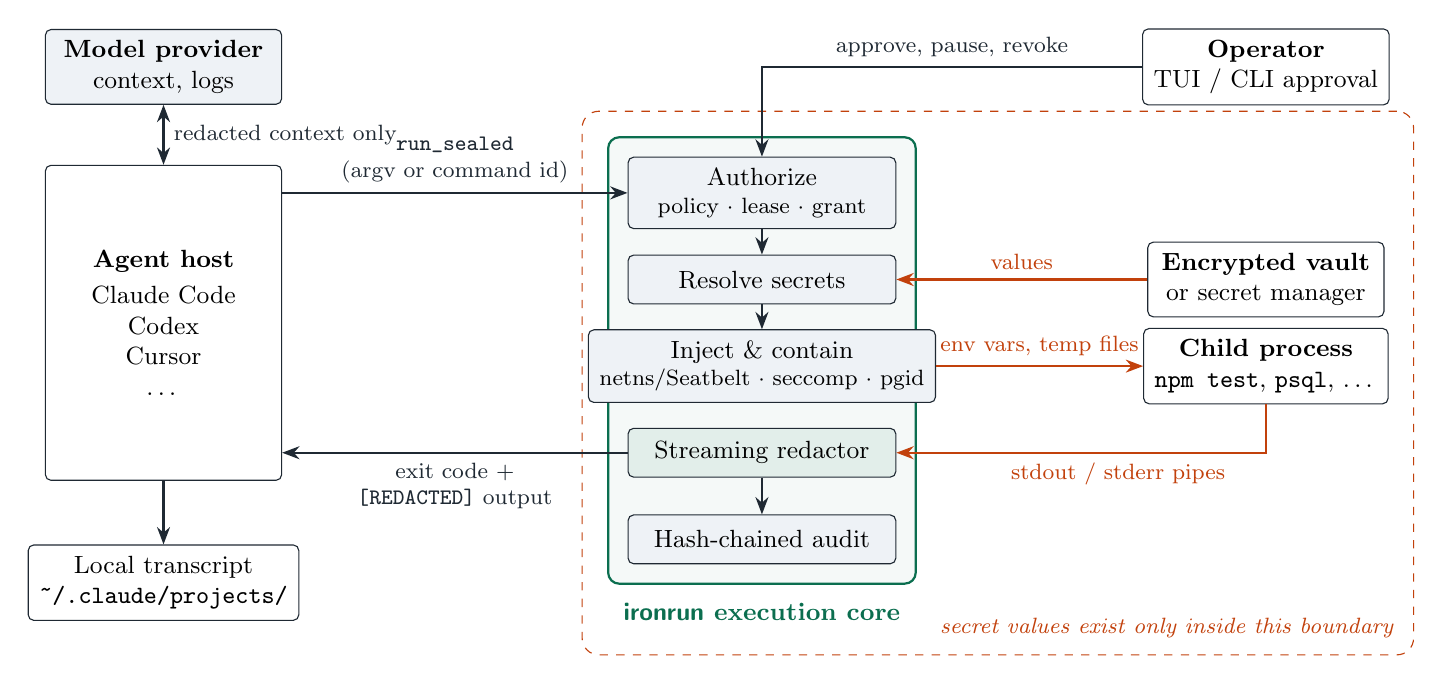
\begin{tikzpicture}[
  font=\small,
  >={Stealth[length=2.2mm]},
  box/.style={draw=ink, rounded corners=2pt, align=center, fill=white, inner sep=4pt},
  stage/.style={box, minimum width=3.4cm, minimum height=0.62cm, fill=soft},
  lab/.style={font=\footnotesize, align=center, text=ink},
  flow/.style={->, thick, draw=ink},
  sflow/.style={->, thick, draw=secret},
]
% ironrun core (stages stacked; y chosen so side arrows are horizontal)
\node[stage] (authz)   at (7.6, 2.4) {Authorize\\[-1pt]\footnotesize policy $\cdot$ lease $\cdot$ grant};
\node[stage] (resolve) at (7.6, 1.3) {Resolve secrets};
\node[stage] (contain) at (7.6, 0.2) {Inject \& contain\\[-1pt]\footnotesize netns/Seatbelt $\cdot$ seccomp $\cdot$ pgid};
\node[stage, fill=accent!12] (redact) at (7.6, -0.9) {Streaming redactor};
\node[stage] (audit)   at (7.6, -2.0) {Hash-chained audit};
\begin{scope}[on background layer]
\node[draw=accent, thick, rounded corners=4pt, fill=accent!4, inner sep=7pt, fit=(authz)(audit)] (core) {};
\end{scope}
\node[font=\small\bfseries, text=accent, anchor=north] (corelabel) at ([yshift=-3pt]core.south) {\sys{} execution core};
\foreach \u/\v in {authz/resolve, resolve/contain, redact/audit} \draw[flow] (\u) -- (\v);

% agent side: one tall box so both arrows to the core are horizontal
\node[box, minimum width=3.0cm, minimum height=4.0cm] (agent) at (0,0.75) {\textbf{Agent host}\\[2pt]Claude Code\\Codex\\Cursor\\\ldots};
\node[box, fill=soft, minimum width=3.0cm] (prov) at (0,4.0) {\textbf{Model provider}\\context, logs};
\node[box, minimum width=3.0cm] (tx) at (0,-2.55) {Local transcript\\\code{~/.claude/projects/}};
\draw[<->, thick, draw=ink] (agent) -- node[lab, right] {redacted context only} (prov);
\draw[flow] (agent) -- (tx);
\draw[flow] (agent.east |- authz.west) -- node[lab, above] {\code{run_sealed}\\(argv or command id)} (authz.west);
\draw[flow] (redact.west) -- node[lab, below] {exit code +\\\red{} output} (agent.east |- redact.west);

% right side
\node[box, minimum width=3.0cm, minimum height=0.9cm] (vault) at (14.0, 1.3) {\textbf{Encrypted vault}\\or secret manager};
\node[box, minimum width=3.0cm, minimum height=0.9cm] (child) at (14.0, 0.2) {\textbf{Child process}\\\code{npm test}, \code{psql}, \ldots};
\node[box, minimum width=3.0cm, minimum height=0.9cm] (human) at (14.0, 4.0) {\textbf{Operator}\\TUI / CLI approval};
\draw[sflow] (vault.west) -- node[lab, above, text=secret] {values} (resolve.east);
\draw[sflow] (contain.east) -- node[lab, above, text=secret] {env vars, temp files} (child.west);
\draw[sflow] (child.south) |- node[lab, below, text=secret, pos=0.7] {stdout / stderr pipes} (redact.east);
\draw[flow] (human.west) -| node[lab, above, pos=0.25] {approve, pause, revoke} (authz.north);

% trust boundary
\begin{scope}[on background layer]
\node[draw=secret, dashed, rounded corners=6pt, inner sep=9pt, fit=(core)(corelabel)(vault)(child)] (tb) {};
\end{scope}
\node[font=\footnotesize\itshape, text=secret, anchor=south east] at ([xshift=-4pt,yshift=3pt]tb.south east) {secret values exist only inside this boundary};
\end{tikzpicture}
\caption{\sys{} architecture. Values (orange) move from the vault into the child
and from the child's pipes into the redactor; they never cross to the agent.
The agent invokes one tool, receives an exit code and redacted output, and
cannot approve its own requests.}
\label{fig:arch}
\end{figure*}

% ---------------------------------------------------------------------------
\subsection{Value-blind interfaces}

The agent-facing MCP server exposes twelve tools (\cref{tab:tools}). Their
schemas are designed so that no field can carry a secret value in either
direction. \code{request_secret}, for example, accepts only a declared alias and
a reason; the human fulfils it through masked local input. If a workflow
requires pasting through chat, the operator instead produces an \emph{encrypted
capsule} (\code{ir1.}\ldots): AES-256-GCM ciphertext under a per-project capsule
key, bound by its authenticated data to the project and by its payload to the
requesting MCP session, request, alias, and a $\leq$10-minute expiry, and usable
once. The plaintext never enters the transcript.

\begin{table}[t]
\centering\small
\begin{tabularx}{\columnwidth}{@{}lX@{}}
\toprule
Tool & Returns (never a value) \\
\midrule
\code{list_commands} & IDs and argv of approved commands \\
\code{run_sealed} & exit code, duration, redacted stdout/stderr \\
\code{request_workspace_access} & request ID for a trusted session \\
\code{workspace_status} & grant state, environment names \\
\code{request_lease} / \code{lease_status} & lease request / state \\
\code{revoke_own_lease} & revocation of the caller's own lease \\
\code{propose_command} & staged proposal ID (runs nothing) \\
\code{request_secret} & request ID (no value field) \\
\code{claim_capsule} & success flag; stores ciphertext's value locally \\
\code{list_environments} & names and key names only \\
\code{validate_policy} & provider and command count \\
\bottomrule
\end{tabularx}
\caption{The agent-facing MCP surface. A guard test fails the build if any tool
result carries vault key material, and removed tools (e.g.\ an earlier
\code{share_environment}) are registered as banned.}
\label{tab:tools}
\end{table}

% ---------------------------------------------------------------------------
\subsection{Authorization tiers}
\label{sec:authz}

\sys{} offers four ways for an agent to obtain secret-bearing execution, ordered
from strictest to most convenient:

\begin{enumerate}
\item \textbf{Strict commands.} The policy file lists exact argv vectors and the
  secrets each receives. The agent calls \code{run_sealed} with a command ID; no
  shell is interposed, so injected values cannot be re-expanded, and argv[0] may
  not be a shell. The policy is re-read on every call.
\item \textbf{Leases.} With \code{require_agent_leases}, a strict command also
  needs an unexpired, unrevoked lease bound to the MCP session, environment, and
  command set (default 1\,h, maximum 24\,h).
\item \textbf{Trusted workspace sessions.} For everyday development, the operator
  grants one MCP session arbitrary-argv execution against one project
  environment for a bounded time (default 2\,h). \code{staging} and \code{prod}
  require separate grants.
\item \textbf{Proposals.} An agent may stage a new strict command with
  \code{propose_command}; it is inert until the operator approves it, at which
  point it is merged into the policy.
\end{enumerate}

Session identifiers are 64-bit values from \code{crypto/rand}, minted per MCP
server process and never accepted from the agent, so a grant cannot outlive the
server instance it was issued to.

\paragraph{Continuation.} A blocked call does not fail; it creates (or reuses) a
deduplicated, value-blind request and waits on persisted state, re-validating
authorization every 100\,ms until the request's deadline
(\cref{fig:seq}). When the operator approves in the TUI, the original call
resumes. This removes the round-trip in which an agent asks the human to
``approve and tell me when done''---a round-trip that, in practice, encourages
humans to paste secrets into chat.

\begin{figure}[t]
\centering
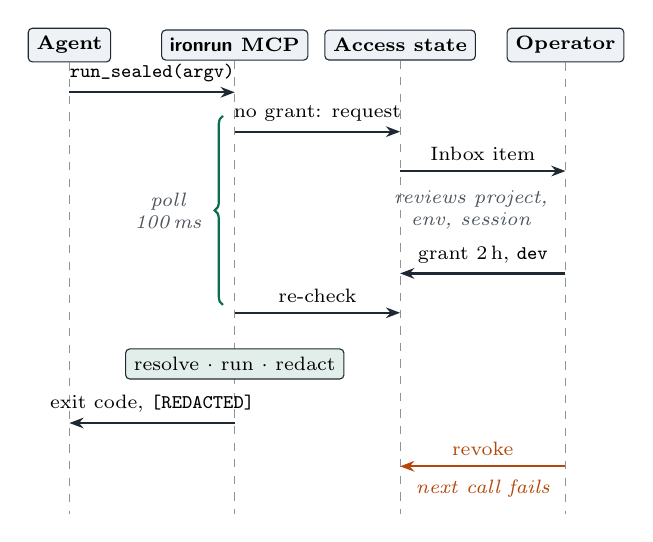
\begin{tikzpicture}[font=\scriptsize, >={Stealth[length=1.8mm]},
  ll/.style={draw=ink!50, dashed},
  hd/.style={draw=ink, rounded corners=1.5pt, fill=soft, inner sep=3pt, align=center, font=\scriptsize\bfseries},
  m/.style={->, thick, draw=ink},
  note/.style={font=\scriptsize\itshape, text=ink!80, align=center}]
\foreach \x/\n/\t in {0/A/Agent, 2.1/M/\sys{} MCP, 4.2/S/Access state, 6.3/H/Operator} {
  \node[hd] (\n) at (\x,0) {\t};
  \draw[ll] (\n.south) -- (\x,-5.95);
}
\draw[m] (0,-0.6) -- node[above] {\code{run_sealed(argv)}} (2.1,-0.6);
\draw[m] (2.1,-1.1) -- node[above] {no grant: request} (4.2,-1.1);
\draw[m] (4.2,-1.6) -- node[above] {Inbox item} (6.3,-1.6);
\node[note, anchor=east] at (6.2,-2.1) {reviews project,\\env, session};
\draw[m] (6.3,-2.9) -- node[above] {grant 2\,h, \code{dev}} (4.2,-2.9);
\draw[thick, draw=accent, decorate, decoration={brace, amplitude=3pt, mirror}] (1.95,-0.9) -- (1.95,-3.3);
\node[note, anchor=east] at (1.8,-2.1) {poll\\100\,ms};
\draw[m] (2.1,-3.4) -- node[above] {re-check} (4.2,-3.4);
\node[hd, fill=accent!12, font=\scriptsize] at (2.1,-4.05) {resolve $\cdot$ run $\cdot$ redact};
\draw[m] (2.1,-4.8) -- node[above] {exit code, \red{}} (0,-4.8);
\draw[m, draw=warn] (6.3,-5.35) -- node[above, text=warn] {revoke} (4.2,-5.35);
\node[note, text=warn, anchor=north] at (5.25,-5.4) {next call fails};
\end{tikzpicture}
\caption{Request, approval, and in-place continuation. The waiting call is never
restarted, and approval happens only on the operator's side.}
\label{fig:seq}
\end{figure}

% ---------------------------------------------------------------------------
\subsection{Resolution and storage}

Secrets come either from an existing manager through its CLI (1Password, HashiCorp
Vault, Doppler, Infisical), from an owner-only env file outside the repository,
or from \sys{}'s own encrypted vault (\cref{fig:keys}). The vault keeps a random
32-byte root key in the OS credential manager. Each environment (a
\emph{scope}) is sealed under a fresh 32-byte data key on every write; the data
key is wrapped by the root key with AES-256-GCM, and both encryptions bind
version, purpose, project, and scope in their authenticated data, so
ciphertexts cannot be moved between environments or projects. The whole
manifest carries an HMAC-SHA256 under the root key and is committed by
write-temp, fsync, rename, and directory fsync. Only names, kinds, and
timestamps are stored unencrypted, under \code{.ironrun/} in the project.

\emph{File secrets} (e.g.\ a service-account JSON) are materialized only for
the duration of a run, in a fresh 0700 directory outside the repository, with
\code{O_EXCL} 0600 files and validated basenames; only the path is injected,
and the contents are registered for redaction.

\begin{figure}[t]
\centering
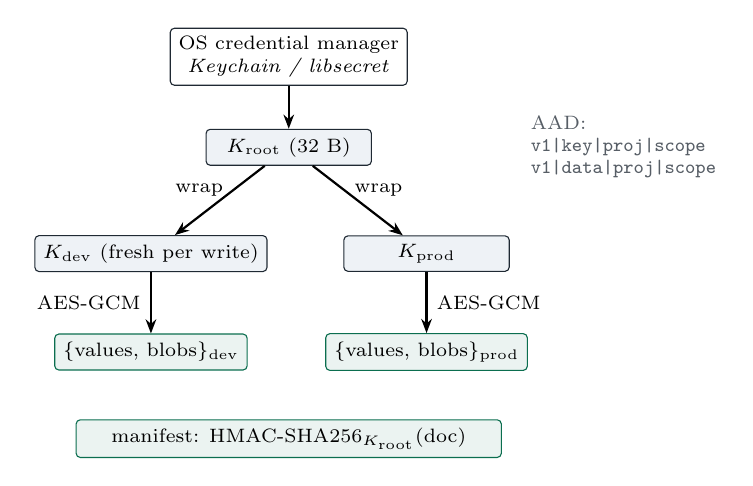
\begin{tikzpicture}[font=\scriptsize, >={Stealth[length=1.8mm]},
  k/.style={draw=ink, rounded corners=1.5pt, fill=soft, align=center, inner sep=3pt, minimum width=2.1cm},
  c/.style={draw=accent, rounded corners=1.5pt, fill=accent!8, align=center, inner sep=3pt}]
\node[k, fill=white] (os) at (0,0) {OS credential manager\\\textit{Keychain / libsecret}};
\node[k] (root) at (0,-1.15) {$K_\mathrm{root}$ (32 B)};
\node[k] (d1) at (-1.75,-2.5) {$K_\mathrm{dev}$ (fresh per write)};
\node[k] (d2) at (1.75,-2.5) {$K_\mathrm{prod}$};
\node[c] (p1) at (-1.75,-3.75) {$\{$values, blobs$\}_\mathrm{dev}$};
\node[c] (p2) at (1.75,-3.75) {$\{$values, blobs$\}_\mathrm{prod}$};
\node[c, minimum width=5.4cm] (mac) at (0,-4.85) {manifest: HMAC-SHA256$_{K_\mathrm{root}}$(doc)};
\draw[->, thick] (os) -- (root);
\draw[->, thick] (root) -- node[left, pos=0.35] {wrap} (d1);
\draw[->, thick] (root) -- node[right, pos=0.35] {wrap} (d2);
\draw[->, thick] (d1) -- node[left] {AES-GCM} (p1);
\draw[->, thick] (d2) -- node[right] {AES-GCM} (p2);
\node[font=\scriptsize, text=ink!75, align=left, anchor=west] at (2.95,-1.15) {AAD:\\\code{v1|key|proj|scope}\\\code{v1|data|proj|scope}};
\end{tikzpicture}
\caption{Vault key hierarchy. Rewriting a scope rotates its data key; AAD binds
every ciphertext to its project and scope.}
\label{fig:keys}
\end{figure}

% ---------------------------------------------------------------------------
\subsection{Streaming known-value redaction}
\label{sec:redact}

Each of the child's output streams passes through its own redacting writer.
Let $V$ be the set of injected values (and file-secret contents) of at least
4 bytes. The writer registers a pattern set
$P = V \cup \bigcup_{v \in V, |v|\geq 8} \mathrm{Enc}(v)$, where $\mathrm{Enc}$
derives the encodings that ordinary tools apply:
base64 (standard and URL alphabets, padded and raw), lower- and upper-case hex,
percent-encoding in the styles of Go, JavaScript, and Python (with
upper- and lower-case escapes), JSON string escaping, second-level nestings
(e.g.\ base64 of base64), base64 wrapped at 64 and 76 columns, and---crucially for
the Basic-auth scenario---the \emph{alignment cores} of base64 at byte offsets
1 and 2 (\cref{sec:align}).

\paragraph{Matching tiers.} At each buffer position the writer tries, in order:
\begin{enumerate}
\item \textbf{Exact}, longest pattern first, using a first-byte index.
\item \textbf{Gap-tolerant}: the pattern's bytes appear in order with
  interleaved whitespace or control bytes ($\leq$\,\code{0x20}, \code{0x7F}),
  which covers terminal line wrapping, \code{\r\n} injection, UTF-16LE
  null interleaving, and one-character-per-line output. The consumed span is
  capped at $2|p|+32$ bytes.
\item \textbf{Fragment}: for patterns with 24 to 65{,}536 non-whitespace bytes,
  every 12-byte window of the pattern's whitespace-free projection is indexed.
  Twelve output bytes that match a window, in order and with any gap bytes
  between them, are extended forward over the rest of the pattern and redacted.
  This catches truncated and partial prints (one line of a PEM key) and
  line-oriented dumps (\code{xxd}, \code{od -c}) whose offset columns cut a
  value into per-line pieces.
\end{enumerate}
A match is replaced by \red{}; unmatched bytes are emitted only once no pattern
could still begin at them.

\paragraph{Bounded hold-back.} Let $m = \max_{p\in P}(2|p|+32)$ be the largest
span any tier may consume. The writer withholds the last $m-1$ bytes of its
buffer until more input arrives or the stream is flushed
(\cref{alg:redact,fig:buffer}).

\begin{algorithm}[t]
\caption{Streaming redaction (one output stream)}
\label{alg:redact}
\small
\begin{algorithmic}[1]
\Procedure{Write}{$x$} \State $B \gets B \,\|\, x$; \Call{Scan}{$m-1$} \EndProcedure
\Procedure{Flush}{} \State \Call{Scan}{$0$} \EndProcedure
\Procedure{Scan}{$h$}
  \While{$|B| > h$}
    \State $i \gets 0$
    \While{$i < |B| - h$ \textbf{and} $\textsc{Match}(B, i) = 0$} \State $i \gets i+1$ \EndWhile
    \State \Call{Emit}{$B[0{:}i]$}; $\ell \gets \textsc{Match}(B,i)$
    \If{$\ell = 0$} \State $B \gets B[i{:}]$; \textbf{break} \EndIf
    \State \Call{Emit}{\red}; $B \gets B[i+\ell{:}]$
  \EndWhile
\EndProcedure
\Function{Match}{$B, i$} \Comment{bytes consumed, $\leq m$}
  \State \Return first nonzero of $\textsc{Exact}$, $\textsc{GapTolerant}$, $\textsc{Fragment}$ at $B[i{:}]$
\EndFunction
\end{algorithmic}
\end{algorithm}

\begin{figure}[t]
\centering
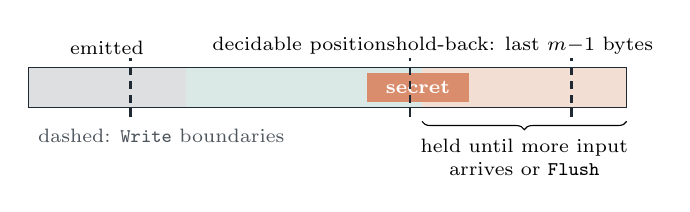
\begin{tikzpicture}[font=\scriptsize]
\fill[ink!15] (0,0) rectangle (2.0,0.5);
\fill[accent!15] (2.0,0) rectangle (5.0,0.5);
\fill[warn!18] (5.0,0) rectangle (7.6,0.5);
\draw[ink] (0,0) rectangle (7.6,0.5);
\node[anchor=south] at (1.0,0.55) {emitted};
\node[anchor=south] at (3.5,0.55) {decidable positions};
\node[anchor=south] at (6.3,0.55) {hold-back: last $m{-}1$ bytes};
\fill[secret!60] (4.3,0.07) rectangle (5.6,0.43);
\node[text=white, font=\scriptsize\bfseries] at (4.95,0.25) {secret};
\foreach \x in {1.3,4.85,6.9} \draw[densely dashed, thick, ink] (\x,-0.12) -- (\x,0.62);
\draw[decorate, decoration={brace, amplitude=3pt, mirror}] (5.0,-0.18) -- (7.6,-0.18)
  node[midway, below=3pt, align=center] {held until more input\\arrives or \code{Flush}};
\node[anchor=north west, align=left, text=ink!80] at (0,-0.15) {dashed: \code{Write} boundaries};
\end{tikzpicture}
\caption{The scanner only decides positions that have at least $m{-}1$ bytes of
lookahead, so a secret that straddles one or more \code{Write} boundaries is
still seen whole.}
\label{fig:buffer}
\end{figure}

\begin{property}[Chunking invariance]
\label{prop:chunk}
For any input $x$ and any partition of $x$ into \code{Write} calls followed by
\code{Flush}, the emitted output equals that of a single \code{Write}$(x)$
followed by \code{Flush}.
\end{property}
\begin{proof}[Proof sketch]
\textsc{Scan} decides position $i$ only if $|B| - i > m - 1$, i.e.\ at least $m$
bytes starting at $i$ are buffered. Every tier inspects at most $m$ bytes from
$i$: exact matching reads $|p| < m$ bytes; gap-tolerant matching is capped at
$2|p|+32 \le m$; fragment lookup and extension are explicitly limited to $m$
bytes. Hence
$\textsc{Match}(B,i)$ depends only on bytes already present and is identical to
its value on the complete input. Positions are decided left to right in the same
order in both executions, and \code{Flush} decides the remaining positions with
the full suffix present. Induction on decided positions gives equal output.
\end{proof}

The cost of this guarantee is latency: up to $m-1$ bytes (a few hundred bytes for
typical tokens) are delayed until the next write or process exit. Interactive
output therefore appears with a short lag, never out of order.

\subsubsection{Base64 alignment}
\label{sec:align}
Base64 maps each 3-byte group to 4 characters. When a secret $s$ of $n$ bytes is
encoded as part of a larger message, the characters that depend \emph{only} on
$s$ are determined by $s$'s offset modulo~3. With $k \in \{0,1,2\}$ bytes of
preceding context, they are
\[
  \mathrm{core}_k(s) = \mathrm{b64}(0^k \| s)\big[\lceil 8k/6 \rceil \,:\, \lfloor 8(k+n)/6 \rfloor\big],
\]
where the trailing bound also drops the final character, which mixes bits of
$s$ with whatever follows. Registering only $\mathrm{b64}(s)$, as \sys{} v0.5.0
did, matches only when $k=0$ and $n \equiv 0 \pmod 3$ and the encoder happens
to stop at $s$; HTTP Basic authentication (\code{user:token}) and
\code{printenv | base64} both violate this two times out of three. Registering
the three cores closes the gap for any surrounding context. The technique is not
new---the GitHub Actions runner has registered shifted base64 forms since
2019~\citep{githubrunner2019encoders}---and its absence from v0.5.0 is one of the
audit findings of \cref{sec:audit}.

% ---------------------------------------------------------------------------
\subsection{Containment}
\label{sec:contain}

Redaction protects the output channel; the following layers bound side effects,
and all of them fail closed:

\begin{itemize}
\item \textbf{Network.} Secret-bearing commands get no network unless the
  policy opts out. On Linux \sys{} enters fresh user and network
  namespaces~\citep{man_userns,man_netns} (\code{CLONE_NEWUSER|CLONE_NEWNET}
  with an identity UID/GID map, so no privilege is needed); on macOS it wraps the
  child in a Seatbelt~\citep{blazakis2011apple} profile that denies only
  \code{network*}, invoking \code{/usr/bin/sandbox-exec}~\citep{apple_sandboxexec}
  by absolute path.
  Unsupported platforms refuse to run.
\item \textbf{Syscalls.} On Linux the child is started through a re-exec shim
  that sets \code{NO_NEW_PRIVS}, installs a seccomp-BPF filter~\citep{linux_seccomp} that checks the
  architecture, rejects the x32 ABI, and returns \code{EPERM} for
  \code{ptrace}, \code{process_vm_readv}/\code{writev}, \code{kcmp},
  \code{perf_event_open}, \code{bpf}, and \code{userfaultfd}, then sets
  \code{RLIMIT_CORE=0} and execs the target in place.
\item \textbf{Lifetime.} The child runs in its own process group; on timeout,
  cancellation, or a signal to \sys{}, the whole group is killed, and any group
  member left after the child exits is killed too, so no descendant outlives the
  run holding secrets in its environment. Temporary file secrets are removed on
  every exit path.
\item \textbf{Environment.} The inherited environment is stripped of loader,
  shell-startup, interpreter, and tool hijack variables (\code{LD_*},
  \code{DYLD_*}, \code{BASH_ENV}, \code{NODE_OPTIONS}, \code{PYTHON*},
  \code{GIT_CONFIG_*}, \code{GOFLAGS}, \ldots) before secrets are added.
\item \textbf{CI.} In GitHub Actions, GitLab CI, CircleCI, and Jenkins, runs
  triggered by fork pull requests (and \code{pull_request_target}, the ``pwn
  request'' pattern~\citep{lobacevski2021pwn,koishybayev2022ci}, without an
  explicit operator flag) are refused before any secret is resolved.
\item \textbf{Operator-only switches.} Every control that weakens protection
  (seccomp, core-dump seal, entropy scan, \code{pull_request_target}) is a
  command-line flag, never an environment variable, because the environment is
  reachable by the agent.
\end{itemize}

\subsection{Audit}
Each run appends a JSONL record---command, argv with all registered patterns
scrubbed, secret names and kinds, redaction count, exit status, sandbox
outcome---whose hash covers the previous record's hash, in the style of
Schneier and Kelsey~\citep{schneier1999audit}. \code{ironrun audit
verify} replays the chain, and a broken chain makes subsequent runs refuse
rather than continue unaudited. The chain is tamper-evident for edits and
reordering; without an external anchor or a Merkle structure~\citep{crosby2009tamper}
it cannot detect truncation of the tail (\cref{sec:discussion}).

% ===========================================================================
\section{Implementation}
\label{sec:impl}

\sys{} is a single static Go binary (17.3\,kLOC of production code, 11.5\,kLOC
of tests across 430 test functions, fuzzing of the redactor) built with
\code{CGO_ENABLED=0}. The MCP server uses \code{mcp-go}. Platforms are macOS and
Linux on amd64 and arm64; Windows is unsupported because its secret-entry paths
would require plaintext console input. Releases are reproducible
(\code{-trimpath}, commit-date timestamps, pinned modules), published with
SHA-256 checksums, an SBOM, and keyless Sigstore bundles~\citep{newman2022sigstore};
the installer and the npm launcher refuse to install an artifact whose checksum
or signature does not verify. The repository runs CodeQL, OpenSSF Scorecard,
\code{govulncheck}, and a scheduled fuzzing job in CI.

% ===========================================================================
\section{Adversarial Self-Audit}
\label{sec:audit}

Before release we audited v0.5.0 (16.6\,kLOC) adversarially. Five reviewers each took one
subsystem---redaction, execution and sandboxing, authorization and agent
surfaces, storage and cryptography, and policy/CLI/distribution---and were
instructed to report only defects backed by an executed probe or a line-level
trace against the documented guarantees. After removing findings reported by
more than one reviewer, 49 distinct defects remained (2 critical, 6 high, 16
medium, 25 low). We fixed 44, each with a regression test that fails on v0.5.0;
the other five follow from the same-user threat boundary or are deliberate
trade-offs, and are documented as limitations (\cref{sec:discussion}). The reviewers were LLM-based code
review agents directed and checked by the authors; we report this because the
method is reproducible and because the class of findings is instructive.
\Cref{tab:audit} summarizes the results.

\begin{table*}[t]
\centering\small
\begin{threeparttable}
\begin{tabularx}{\textwidth}{@{}llXl@{}}
\toprule
ID & Sev. & Finding & Resolution \\
\midrule
\multicolumn{4}{@{}l}{\emph{Agent surfaces and authorization}} \\
A1 & High & Proposal approval spliced agent text (reason, env names/refs, v2 secret names) into \code{ironrun.yml} unescaped; a newline---or U+2028, which YAML also treats as a line break---smuggled extra commands past human review & fixed \\
A2 & Med & Approval bound to a proposal ID whose content the agent could replace between display and approval & fixed \\
A3 & Med & Approval display lost argv boundaries, passed control characters to the terminal, and hid v1 secret references in the TUI & fixed \\
A4 & Med & A trusted session can run \sys{} itself to grant or extend its own access & documented \\
A5 & Low & \code{propose_command} and the local API used the startup policy, delaying revocation & fixed \\
\multicolumn{4}{@{}l}{\emph{Storage and cryptography}} \\
S1 & Crit & \code{ironrun env share} printed the vault root key to stdout, with no gate & fixed (removed) \\
S2 & High & \code{env sync pull} overwrote the vault with unverified remote bytes (data loss, rollback) & fixed \\
S3 & Med & Root key passed on the \code{security} command line (visible to process listings and EDR) & fixed \\
S4 & Med & Audit log failed open on tamper detection; tail truncation undetected & fixed / documented \\
S5 & Med & Equivalent remote URLs (HTTPS vs.\ SSH) changed project identity and locked users out & fixed \\
S6 & Low & No anti-rollback for vault copies; lost metadata updates under concurrency & documented / fixed \\
\multicolumn{4}{@{}l}{\emph{Redaction}} \\
R1 & Crit & GitHub mask emission printed lines 2..$N$ of multi-line secrets (PEM keys, service-account JSON) to job logs in cleartext & fixed \\
R2 & High & Base64 matched only at offset 0 (Basic auth, docker \code{auth}, \code{printenv|base64} leaked) & fixed \\
R3 & High & No fragment coverage for secrets over 1\,KiB (partial prints of PEM/JSON file secrets leaked) & fixed \\
R4 & Med & Hex dumps (\code{xxd}, \code{hexdump -C}, \code{od -c}) defeated hex coverage & fixed \\
R5 & Med & Only Go's URL escapers covered; JSON-escaped forms missed (incl.\ in transcript scrubbing) & fixed \\
\multicolumn{4}{@{}l}{\emph{Execution and sandboxing}} \\
E1 & High & TTL not enforced when a grandchild held the output pipe; descendants outlived the run with secrets & fixed \\
E2 & Med & A signal to \sys{} left plaintext file secrets on disk and orphaned the child & fixed \\
E3 & High & macOS network sandbox also denied \code{fork}, breaking most real commands; the macOS network test passed vacuously & fixed \\
E4 & Med & \code{sandbox-exec} resolved through \code{PATH}, letting the environment disable isolation & fixed \\
E5 & Low & Relative \code{workdir} resolved against the caller's cwd instead of the project root & fixed \\
E6 & Low & Shell denylist bypassable by path variants (\code{/bin//sh}); env denylist gaps (\code{GOFLAGS}, \code{GIT_CONFIG_*}) & fixed \\
\multicolumn{4}{@{}l}{\emph{Policy, CLI, and distribution}} \\
P1 & Med & GitHub fork-PR detection compared a variable GitHub never sets, so fork runs were trusted; secrets were resolved and masks printed before the gate & fixed \\
P2 & Med & Git hooks were installed where git does not read them (linked worktrees, \code{core.hooksPath}); hook scanning missed multi-line and binary values and non-active environments & fixed \\
P3 & Med & The next stable release would fail before signing (missing tap token); the npm package could not be installed & fixed \\
P4 & Low & Third-party actions in the signing workflow were pinned by mutable tag & fixed (SHA) \\
P5 & Low & Dotenv and envfile parsing corrupted values and paths; policy \code{env:} keys unvalidated & fixed \\
\bottomrule
\end{tabularx}
\begin{tablenotes}\footnotesize
\item Lower-severity items (exit-code reporting, truncation flags, backup files left by history purge, import-guard path handling) were also fixed and are listed in the changelog.
\end{tablenotes}
\end{threeparttable}
\caption{Defects confirmed by the self-audit of v0.5.0.}
\label{tab:audit}
\end{table*}

\paragraph{Lesson 1: human-in-the-loop is only as strong as what the human sees.}
A1--A3 share a root cause: approval rendered agent-controlled text into a second
language (YAML) by string concatenation, and showed it to the human through a
third (a terminal). The reviewer saw a ``reason''; the parser saw a command.
The fix quotes every agent-derived scalar, flattens comments to a single line
under YAML's definition of a line break (which includes NEL, U+2028, and
U+2029), rejects multi-line text at the MCP boundary, makes pending proposals
immutable, and shows argv with explicit element boundaries. The general rule is
that an approval UI must display the \emph{parsed} artifact that will be
enforced, not the text that produced it.

\paragraph{Lesson 2: value-blindness is a property of every surface the agent
can reach.} The project had removed an MCP tool that returned the root key and
added a guard test against its return---but the equivalent CLI command remained,
and agents have shells. S1 and R1 are both instances of a value leaving through
a surface designed for humans or CI. We now treat the CLI as agent-reachable
and test it accordingly.

\paragraph{Lesson 3: encodings have structure.} R2 is not a missing encoding but
a missing \emph{alignment}; R4 and R5 are formatting conventions of specific
tools. Enumerating ``base64'' as a single transformation was the error.

\paragraph{Lesson 4: fail-closed tests can pass for the wrong reason.} The
macOS network test asserted a non-zero exit, which the sandbox produced by
crashing the probe before it dialed (E3). The corrected test distinguishes
``connection refused by policy'' from ``process failed''.

% ===========================================================================
\section{Evaluation}
\label{sec:eval}

We ask: \textbf{RQ1} how much of a secret reaches the agent under realistic and
adversarial output transformations; \textbf{RQ2} how often benign output is
redacted; \textbf{RQ3} what the runtime costs; and \textbf{RQ4} whether
streaming behaves exactly like batch processing. All numbers come from the
open harness in \code{paper/eval} on an Apple M3 Pro (macOS 26.4, Go 1.26.5).

\paragraph{Method (RQ1).} We generate six synthetic credentials shaped like real
formats: a Stripe-style key (32\,B), a GitHub PAT (40\,B), an AWS-style secret
(40\,B), a Postgres URL with an embedded password (68\,B), a 12-byte password,
and a JWT (114\,B). For each of 21 transformations we write the transformed
output to a file and have a real child (\code{cat}) print it through
\code{runner.Run} with the secret injected---the same injection, pipe,
registration, and redaction path a sealed run uses. We then attack the
agent-visible output with a decoder battery: identity, gap stripping, case
folding, reversal, ROT13, base64 and hex decoding at every alignment (with
nesting and gunzip), URL and JSON unescaping, and hexdump column reassembly.
\emph{Recovered} is the longest contiguous run of secret bytes any decoder
yields; a case \emph{leaks} if at least 50\% of the secret is recovered.

\begin{table}[t]
\centering\small
\setlength{\tabcolsep}{4pt}
\begin{tabular}{@{}llcc@{}}
\toprule
Transformation & Class & v0.5.0 & Fixed \\
\midrule
\code{printenv} line & acc. & 0/6 & 0/6 \\
\code{set -x} trace & acc. & 0/6 & 0/6 \\
JSON (Go encoder) & acc. & 1/6 & \textbf{0/6} \\
URL query parameter & acc. & 0/6 & 0/6 \\
HTTP Basic auth & acc. & 6/6 & \textbf{0/6} \\
k8s Secret (base64) & acc. & 0/6 & 0/6 \\
\code{printenv | base64} & acc. & 6/6 & \textbf{0/6} \\
\code{xxd} hexdump & acc. & 6/6 & \textbf{1/6} \\
ANSI-highlighted & acc. & 1/6 & 1/6 \\
pty wrap (CRLF) & acc. & 0/6 & 0/6 \\
UTF-16LE & acc. & 0/6 & 0/6 \\
truncated (first 60\%) & acc. & 1/6 & 1/6 \\
\midrule
hex & del. & 0/6 & 0/6 \\
base64 at offset 1 & del. & 6/6 & \textbf{0/6} \\
double base64 & del. & 0/6 & 0/6 \\
gzip $|$ base64 & del. & 6/6 & 6/6 \\
one char per line & del. & 0/6 & 0/6 \\
split with separator & del. & 1/6 & 1/6 \\
reversed & del. & 6/6 & 6/6 \\
ROT13 & del. & 6/6 & 6/6 \\
upper-cased & del. & 6/6 & 6/6 \\
\midrule
\textbf{Accidental} & & \textbf{21/72} & \textbf{3/72} \\
\textbf{All} & & \textbf{52/126} & \textbf{28/126} \\
\bottomrule
\end{tabular}
\caption{Secrets (of 6) of which $\geq$50\% is recoverable from agent-visible
output, before and after the audit fixes. \emph{acc.}: produced by ordinary
tools; \emph{del.}: deliberate.}
\label{tab:leak}
\end{table}

\paragraph{Results (RQ1).} \Cref{tab:leak} shows that v0.5.0 already handled
literal prints, xtrace, URL parameters, aligned base64, wrapping, CRLF,
UTF-16, and nested encodings, but leaked every secret under three
\emph{accidental} transformations---Basic auth, \code{printenv | base64}, and
\code{xxd}---for the alignment and formatting reasons of \cref{sec:audit}.
After the fixes, every accidental transformation is closed for all credentials
of 24 bytes or more. The three remaining accidental cases all involve the
12-byte password, which is below the fragment threshold: a 60\% prefix, a
color escape in the middle of the value, and the \code{xxd} ASCII column, which
prints it in two pieces.

Four deliberate transformations remain out of reach, and necessarily so:
\begin{observation}
\label{obs:arbitrary}
For any finite set of registered encodings, an authorized process that applies
an unregistered invertible transformation $f$ (reversal, ROT13, XOR with a
constant, compression) to a secret and prints the result defeats known-value
redaction, since $f(s)$ shares no registered pattern with $s$.
\end{observation}
Redaction is therefore a defense against A1, not against an A2 that can choose
the program. Against A2, \sys{} relies on the strict tier (the agent cannot
choose the program), on network isolation (the transformed secret cannot leave
except through output), and on the warn-only entropy scan, which flagged
21 of the 28 residual leaks (and none of the redacted cases). Compression is the instructive exception:
gzip output is binary and therefore unreadable in a transcript, yet trivially
decodable, which is why it is in the corpus.

\paragraph{RQ2: false positives.} We run the redactor over 1.0\,MB of benign
text (the repository's own sources and documentation, plus 1,000 log lines that
share structure with a connection URL) with each credential and its full
encoding set registered (\cref{tab:fp}). Random-format credentials produced no
false positives. The structured Postgres URL produced 1,002 both before and after the fixes: its non-secret
12-byte windows (\code{db.internal:5432/app}) occur in ordinary logs and
trigger the fragment tier. Over-redaction is safe but degrades output; we
discuss mitigations in \cref{sec:discussion}.

\begin{table}[t]
\centering\small
\begin{tabular}{@{}lrrr@{}}
\toprule
Credential & Patterns$^\dagger$ & FP (v0.5.0) & FP (fixed) \\
\midrule
Stripe key & 18 & 0 & 0 \\
GitHub PAT & 18 & 0 & 0 \\
AWS secret & 18 & 0 & 0 \\
Postgres URL & 22 & 1,002 & 1,002 \\
password (12\,B) & 14 & 0 & 0 \\
JWT & 22 & 0 & 0 \\
\bottomrule
\end{tabular}
\caption{Redactions on 1.0\,MB of benign text (all are false positives).
$^\dagger$Registered patterns per credential after the fixes.}
\label{tab:fp}
\end{table}

\paragraph{RQ3: overhead.} Spawning \code{true} directly takes a median
1.60\,ms; through \code{runner.Run} with one secret it takes 1.68\,ms
(+0.08\,ms), and with macOS network isolation 7.37\,ms, dominated by
\code{sandbox-exec} start-up ($n{=}200$, fixed version). Registering the new
encodings raises the patterns per 40-byte credential from 15 to 18 and lowers
single-secret throughput from 56 to 35\,MB/s; both remain far above
interactive output rates. Provider look-ups add their own
latency (e.g.\ a 1Password CLI call). \Cref{fig:throughput} reports redactor
throughput on 4\,MiB of log text written in 32\,KiB chunks.

\begin{figure}[t]
\centering
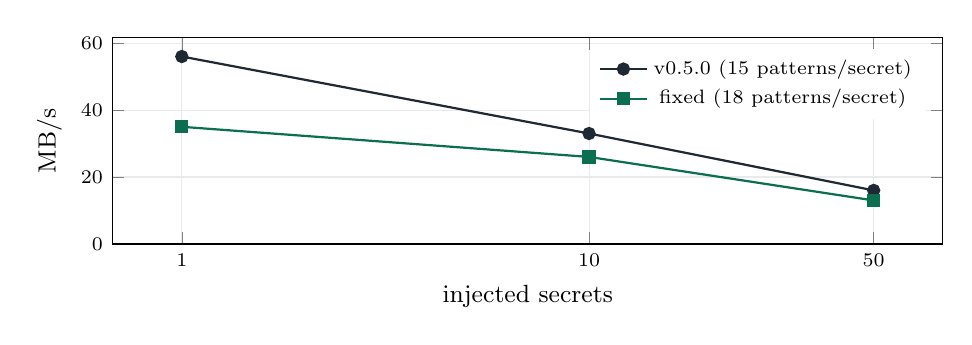
\begin{tikzpicture}
\begin{axis}[width=\columnwidth, height=4.2cm, xmode=log, log basis x=10,
  xlabel={injected secrets}, ylabel={MB/s}, xtick={1,10,50}, xticklabels={1,10,50},
  ymin=0, legend style={font=\scriptsize, draw=none, at={(0.98,0.95)}, anchor=north east},
  tick label style={font=\scriptsize}, label style={font=\small}, grid=major, grid style={ink!10}]
\addplot[mark=*, thick, color=ink] coordinates {(1,56) (10,33) (50,16)};
\addlegendentry{v0.5.0 (15 patterns/secret)}
\addplot[mark=square*, thick, color=accent] coordinates {(1,35) (10,26) (50,13)};
\addlegendentry{fixed (18 patterns/secret)}
\end{axis}
\end{tikzpicture}
\caption{Redactor throughput. Terminal-scale output is far below either curve.}
\label{fig:throughput}
\end{figure}

\paragraph{RQ4: streaming equivalence.} \Cref{prop:chunk} is exercised by a
differential test that feeds 3,000 random inputs (secrets, their encodings,
gap-interleaved and fragmentary forms) through the writer in chunks of 1, 2, 3,
7, and 13 bytes and compares against a single write; no divergence was observed
before or after the fixes. The repository additionally fuzzes the writer
continuously in CI.

% ===========================================================================
\section{Discussion and Limitations}
\label{sec:discussion}

\paragraph{Substitution is stronger than redaction.} In proxy-substitution
designs the child holds only a placeholder and a proxy inserts the real value
into outbound HTTP(S) requests~\citep{claudecode_sandboxing,infisical_agentproxy,onecli2026,cyberark_secretless},
so no output transformation can reveal it. Where that applies, it should be
preferred. It does not apply to the many tools that use credentials outside
HTTP---database wire protocols, SSH, signing keys, file-based service-account
credentials---which is the space \sys{} targets; the two compose.

\paragraph{Redaction is a safety net, not a sandbox.} \Cref{obs:arbitrary} is
fundamental. \sys{}'s strongest configuration---strict commands, leases, and no
network---lets the agent choose \emph{when} to run a reviewed program but not
\emph{what} it computes. Trusted workspace sessions trade this away for
convenience: the agent chooses argv, receives every entry of the environment in
the child, and could deliberately encode a secret. We document trusted sessions
as protecting context and logs from accidents, not as containment.

\paragraph{State integrity against A2.} Authorization state (\code{.ironrun/},
\code{ironrun.yml}) lives in the project, where an agent with file-edit tools
can write it, and a trusted session can run \sys{} itself (A4). Same-user
storage cannot protect itself from same-user code. The principled remedy is to
move approvals and state behind a broker running as a different user, with the
agent host's own file and command restrictions guarding the checkout in the
meantime.

\paragraph{Credential-store reachability.} Keychain items created through
\code{/usr/bin/security} are readable by any same-user process that invokes it,
and the legacy file store keeps its key beside its ciphertext. Both are
consistent with the A3 exclusion but matter for A2 with an unrestricted shell.

\paragraph{Audit truncation and vault rollback.} The hash chain and the vault
manifest MAC detect modification but not replacement by an older valid state.
Anchoring the latest chain head and vault revision in the OS credential manager
would give monotonicity against everything short of A3.

\paragraph{Partial and structured secrets.} A short secret ($<$24\,B) printed
partially---say its first seven characters---is not fragment-indexed, and a
structured secret's boilerplate windows cause over-redaction (\cref{tab:fp}).
Both trace to treating every 12-byte window alike; weighting windows by
estimated entropy, or decomposing URLs into their userinfo component, are
natural refinements.

\paragraph{Platform.} macOS's \code{sandbox-exec} is deprecated though
functional; Windows is unsupported. Provider-side retention of anything that
\emph{did} reach context is outside \sys{}'s reach.

% ===========================================================================
\section{Related Work}
\label{sec:related}

\paragraph{Prompt injection and agent security.} Indirect prompt
injection~\citep{greshake2023youve,perez2022ignore} and its formalization and
benchmarks~\citep{liu2024formalizing,debenedetti2024agentdojo,zhan2024injecagent}
establish that an agent's behavior can be steered by data it reads, and adaptive
attacks defeat most model-level defenses~\citep{nasr2025attacker}. Willison's
``lethal trifecta''~\citep{willison2025trifecta} and Meta's ``rule of
two''~\citep{meta2025ruleoftwo} frame exfiltration as the conjunction of private
data, untrusted input, and an outbound channel. \sys{} removes the first from
the agent's view and, with network isolation, the third from the child.

\paragraph{System-level defenses.} CaMeL~\citep{debenedetti2025camel},
design patterns for injection-resistant agents~\citep{beurerkellner2025design},
information-flow control~\citep{costa2025fides,wu2024fsecure}, privilege
policies~\citep{shi2025progent}, and execution isolation~\citep{wu2025isolategpt},
building on the dual-LLM pattern~\citep{willison2023dual}, constrain what a
compromised planner can do. \sys{} is narrower and deterministic: one data class
(credentials), one sink (tool output), no change to the model or planner. Its
redactor is a fixed declassification rule at a single boundary, and its strict
mode corresponds to the action-selector pattern at the shell level. A recent
systematization of execution security for coding agents finds deny-lists failing
at high rates~\citep{rashidi2026balkanization}, consistent with our
allow-list-first design.

\paragraph{MCP security.} Measurement and attack studies of the MCP
ecosystem~\citep{hou2025mcplandscape,hasan2025mcpfirstglance,zhao2026parasites,guo2025mcpmeasurement,chen2026rethinkingmcp,zhou2026mcpauth}
document tool poisoning~\citep{invariant2025toolpoisoning,wang2026mcptox},
credential theft through MCP-connected tools~\citep{radosevich2025mcpsafety},
bidirectional data-flow risks~\citep{hou2026unsafeflow}, and context leaking into
tool arguments of coding agents~\citep{xie2025toolleak}. \sys{} sits on the
return path of a local stdio server and assumes a possibly poisoned agent.

\paragraph{Secret leakage and detection.} Secrets leak widely in public
code~\citep{meli2019git}, code models can memorize them~\citep{huang2024codesecret},
and vendor data suggest AI-assisted commits leak more often than
average~\citep{gitguardian2025sprawl,gitguardian2026sprawl}. Pattern-based
detectors trade precision for recall~\citep{basak2023comparative,basak2023secretbench};
\sys{} sidesteps detection by matching only values it injected. Closest in the
literature, Kenney et al.\ evaluate a vault-mediated boundary for API
connectors and conclude that output redaction is a separate, necessary
layer~\citep{kenney2026vault}, and SlotGuard substitutes \emph{detected}
secrets at the transcript boundary~\citep{xia2026slotguard}. Chen et al.\
identify stdout-to-context as the dominant leak path in agent skills without
proposing a runtime fix~\citep{chen2026skillsleak}.

\paragraph{CI log masking.} The GitHub Actions runner masks registered secrets
and automatically derived forms---base64 at all three alignments, URI, JSON, XML,
and shell escapes---in job logs~\citep{githubrunner2019encoders}, while noting
that masking relies on exact matches and is not guaranteed~\citep{github2026secureuse}.
\sys{} adopts this idea for an interactive, streaming setting and adds
whitespace-tolerant and fragment matching; we also found that its own
integration with GitHub's line-oriented mask command could leak multi-line
values (R1).

\paragraph{Industry tools.} Run wrappers inject
secrets~\citep{onepassword_oprun,doppler_cli,infisical_run}, and \code{op run}
also conceals them in output. Agent access products broker
credentials~\citep{onepassword2026unified,bitwarden2026agentaccess}; Doppler's
MCP server deliberately exposes values to agents~\citep{doppler_mcp} and
Infisical's can mask values in its own responses~\citep{infisical_mcp}.
Proxy substitution keeps values out of processes for
HTTP(S)~\citep{claudecode_sandboxing,infisical_agentproxy,onecli2026,flyio_tokenizer,cyberark_secretless}.
The nearest tools to \sys{} are fnox's MCP \code{exec}, which injects secrets
and redacts their literal values from output~\citep{fnox_mcp}, and Prismor's
Cloak, which substitutes placeholders through agent-host hooks and scrubs
literal values~\citep{prismor2026}. Pattern-based scanners and gateways inspect
tool traffic~\citep{ggshield_aihook,truefoundry_secrets,mcpguard2026,redactmcp2026},
and other tools scrub traces or histories after the
fact~\citep{langwatch_redaction,agentsweep2026}. Agent hosts now expose hooks
that can rewrite tool output~\citep{claudecode_hooks} and ship their own
sandboxes~\citep{claudecode_sandboxing,anthropic_srt}. \sys{} differs in
combining encoding-, alignment-, whitespace-, and fragment-aware known-value
redaction with session-bound authorization and OS containment for arbitrary
programs, and in evaluating that redaction adversarially.

\paragraph{Isolation and integrity primitives.} Heavier isolation via
user-space kernels or microVMs~\citep{young2019gvisor,agache2020firecracker} and
unprivileged sandboxes~\citep{bubblewrap} would strengthen containment at a
cost; \sys{} uses namespaces, seccomp, and Seatbelt to stay a single
dependency-free binary. Release signing follows Sigstore~\citep{newman2022sigstore}.

% ===========================================================================
\section{Conclusion}
\label{sec:conclusion}

Coding agents need to use credentials far more often than they need to know
them. \sys{} makes the tool boundary a one-way valve: secrets enter child
processes, and their literal and encoded forms are stripped from everything
that returns. A streaming known-value redactor with a provable chunking
property, session-bound human authorization with in-place continuation, and
fail-closed containment together remove the common accidental-disclosure paths
at a cost of well under a millisecond of redaction per command. Our self-audit
shows where such systems actually break---in the rendering of what humans
approve, in surfaces built for humans that agents can also reach, and in the
structure of encodings---and our measurements make the boundary of known-value
redaction explicit. \sys{} is available under the MIT license at
\url{https://github.com/Generalized-Labs/ironrun}.

\paragraph{Availability.} The evaluation harness (\code{go run ./paper/eval})
regenerates every number in \cref{sec:eval}; \code{make -C paper} builds this
document.

\paragraph{Disclosure.} Portions of the audit and of this manuscript's
preparation were assisted by LLM-based tools under the authors' direction; all
findings were confirmed by executed probes or manual review, and all claims were
checked against the code.

\bibliographystyle{plainnat}
\bibliography{references}

\end{document}
